\documentclass[10pt,a4paper]{article}
\usepackage[left=2cm,right=2cm,top=2cm,bottom=2cm]{geometry}
\usepackage[T1]{fontenc}
\usepackage{lmodern}
\usepackage[spanish,es-tabla,es-noquoting]{babel}
\usepackage[dvipsnames]{xcolor}
\usepackage[fleqn]{mathtools}
\usepackage{booktabs}
\usepackage{amsmath}
\usepackage{latexsym}
\usepackage{graphicx}
\usepackage{nccmath}
\usepackage{multicol}
\usepackage{listings}
\usepackage{tasks}
\usepackage{color}
\usepackage{float}
\usepackage{array}
\usepackage{tikz}
\usetikzlibrary{arrows.meta}
\usepackage{csquotes}
\usepackage[backend=biber,style=numeric,sorting=none]{biblatex}
\addbibresource{referencias.bib}

\definecolor{colorIPN}{rgb}{0.5, 0.0,0.13}
\definecolor{colorESCOM}{rgb}{0.0, 0.5,1.0}
\graphicspath{ {imagenes/} }

\begin{document}
%#########################################################
\begin{titlepage}
	\centering
	{ \huge \bfseries \color{colorIPN}{Instituto Politécnico Nacional} \par}
	{ \Large \bfseries  \color{colorESCOM}{Escuela Superior de Cómputo} \par }
	\vspace{1cm}
	{\huge\Large \color{colorIPN}{Web Client and Backend Development Frameworks}.\par}
	\vspace{1.5cm}
	{\huge\Large  \color{colorESCOM}{Práctica: CRUD de Carrera con JDBC, el patrón DAO y procedimientos almacenados (CallableStatement)}\par}
		\vspace{2cm}
	{\Large\itshape \color{colorIPN}{Profesor: Dr. José Asunción Enríquez Zárate}\par} \hfill \break
	\vspace{2cm}
	{\Large\itshape \color{colorIPN}{Alumno: Angel Frausto Robles}\par} \hfill \break
	{\Large\itshape \color{colorIPN}{Boleta: 2019630177}\par} \hfill \break
	{\Large\itshape \color{colorIPN}{id634296@gmail.com}\par} \hfill \break
	{\Large\itshape \color{colorIPN}{7CM2} \par}
	\vfill
	{\large \color{colorIPN}{\today}\par}
	\vfill
\end{titlepage}

\renewcommand\lstlistingname{Código}

\lstset{
	basicstyle=\small\sffamily,
	numbers=left,
	numberstyle=\tiny,
	frame=tb,
	tabsize=4,
	columns=fixed,
	showstringspaces=false,
	showtabs=false,
	keepspaces,
	commentstyle=\color{Violet},
	keywordstyle=\color{colorIPN} \bfseries,
	stringstyle=\color{colorESCOM},
	extendedchars=true,
	inputencoding=utf8,
	literate=
		{á}{{\'a}}1 {é}{{\'e}}1 {í}{{\'i}}1 {ó}{{\'o}}1 {ú}{{\'u}}1
		{Á}{{\'A}}1 {É}{{\'E}}1 {Í}{{\'I}}1 {Ó}{{\'O}}1 {Ú}{{\'U}}1
		{ñ}{{\~n}}1 {Ñ}{{\~N}}1 {ü}{{\"u}}1 {¿}{{?`}}1 {¡}{{!`}}1
}

\settasks{
	counter-format=(tsk[r]),
	label-width=4ex
}
\tableofcontents
\pagebreak
\listoffigures
\pagebreak
\listoftables
\pagenumbering {arabic}

\pagebreak

%################################################
\section{\color{colorIPN}{Introducción}}

Esta práctica conecta una aplicación de escritorio en Java con MySQL a través de JDBC. El acceso a datos sigue el patrón DAO y el SQL vive en la base como cinco procedimientos almacenados (\textit{stored procedures}), que \texttt{CarreraDAO} invoca con \texttt{CallableStatement}. La ventana Swing (\texttt{VentanaCarrera}) solo llama a los cinco métodos del DAO.

%################################################
\section{\color{colorIPN}{Desarrollo de la aplicación}}

\subsection{La tabla en la base de datos}

La base \texttt{MisCursos} corre en un contenedor de MySQL 8.0 (\texttt{docker-compose.yml} del proyecto), publicado en el puerto 3307 del equipo. Al crearse el contenedor por primera vez se ejecutan, en orden, los dos scripts de la carpeta \texttt{init/}: \texttt{01-schema.sql} crea la tabla y \texttt{02-procedimientos.sql} crea los procedimientos. La figura \ref{img:describe} muestra la estructura de la tabla con \texttt{describe Carrera;}. El campo \texttt{nombreCarrera} es \texttt{UNIQUE}, lo que más adelante produce el error de la figura \ref{img:duplicado}.

\begin{figure}[H]
	\centering
	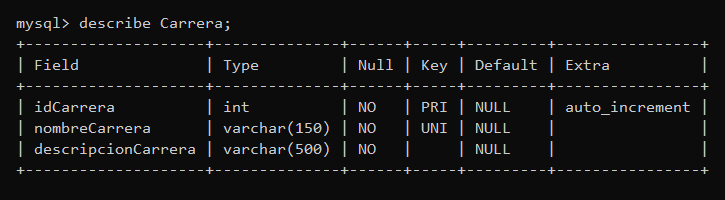
\includegraphics[width=0.8\linewidth]{00_describe_carrera.png}
	\caption{Estructura de la tabla Carrera (\texttt{describe Carrera;})}
	\label{img:describe}
\end{figure}

\subsection{Las clases DTO y DAO}

\textbf{DTO (\texttt{Carrera}).} Es un objeto de transferencia de datos: solo guarda los tres atributos de la tabla (\texttt{idCarrera}, \texttt{nombreCarrera} y \texttt{descripcionCarrera}), todos privados, con sus \textit{getters} y \textit{setters} y un \texttt{toString}. No contiene lógica ni sabe nada de SQL. Es lo que viaja entre la ventana y el DAO.

\textbf{DAO (\texttt{CarreraDAO}).} Concentra todo el acceso a la base de datos \cite{alur2003corej2ee}. Expone cinco métodos públicos (\texttt{create}, \texttt{read}, \texttt{readAll}, \texttt{update} y \texttt{delete}) y un método privado, \texttt{obtenerConexion()}, que carga el driver y abre la conexión JDBC. La ventana solo importa \texttt{SQLException} de \texttt{java.sql}, para atrapar los errores que declara el DAO y mostrarlos en un cuadro de diálogo. No abre conexiones ni arma consultas.

\begin{lstlisting}[caption={Conexión JDBC en CarreraDAO (\texttt{obtenerConexion})}]
private void obtenerConexion() throws SQLException {
    String usuario = "root";
    String clave = "tu_password";
    String urlBD = "jdbc:mysql://localhost:3307/MisCursos";
    String driverMySQL = "com.mysql.cj.jdbc.Driver";

    try {
        Class.forName(driverMySQL);
    } catch (ClassNotFoundException e) {
        throw new SQLException("No se encontro el driver de MySQL: "
                               + driverMySQL, e);
    }
    conexion = DriverManager.getConnection(urlBD, usuario, clave);
}
\end{lstlisting}

La URL apunta al puerto 3307 y a la base \texttt{MisCursos}. El driver es el conector de MySQL (Connector/J) \cite{mysql_connectorj}, que debe estar en el \textit{classpath} al compilar y ejecutar. Si no lo está, \texttt{ClassNotFoundException} se convierte en \texttt{SQLException}, de modo que todo el DAO declara un único tipo de error.

\subsection{Los procedimientos almacenados}

Un procedimiento almacenado es un bloque de SQL guardado en el servidor con un nombre y parámetros, que se ejecuta con \texttt{CALL} \cite{mysql_create_procedure}. Se creó uno por cada operación del CRUD (código \ref{lst:sql}). Todos los parámetros son de entrada (\texttt{IN}). Como el cuerpo de cada procedimiento contiene puntos y coma, el script cambia temporalmente el delimitador a \texttt{\$\$} con \texttt{DELIMITER}; si no, el cliente cortaría la sentencia en el primer \texttt{;}.

\lstinputlisting[language=SQL,caption={Los cinco procedimientos almacenados (\texttt{init/02-procedimientos.sql})},label={lst:sql}]{../init/02-procedimientos.sql}

\begin{table}[H]
	\centering
	\small
	\setlength{\tabcolsep}{4pt}
	\begin{tabular}{@{}llll@{}}
		\toprule
		Operación & Método del DAO & Procedimiento & Sentencia interna \\
		\midrule
		Alta & \texttt{create} & \texttt{sp\_crear\_carrera(nombre, descripcion)} & \texttt{INSERT} \\
		Consulta por id & \texttt{read} & \texttt{sp\_leer\_carrera(id)} & \texttt{SELECT ... WHERE} \\
		Consulta general & \texttt{readAll} & \texttt{sp\_listar\_carreras()} & \texttt{SELECT} \\
		Cambio & \texttt{update} & \texttt{sp\_actualizar\_carrera(id, nombre, descripcion)} & \texttt{UPDATE} \\
		Baja & \texttt{delete} & \texttt{sp\_eliminar\_carrera(id)} & \texttt{DELETE} \\
		\bottomrule
	\end{tabular}
	\caption{Correspondencia entre las operaciones del CRUD, los métodos del DAO y los procedimientos}
	\label{tab:correspondencia}
\end{table}

La figura \ref{img:procs} muestra que los cinco procedimientos existen en la base, consultados en \texttt{information\_schema}. La figura \ref{img:calls} los ejecuta directamente desde el cliente de MySQL, sin pasar por Java: \texttt{sp\_listar\_carreras} y \texttt{sp\_leer\_carrera(1)} devuelven el registro que dejó la aplicación.

\begin{figure}[H]
	\centering
	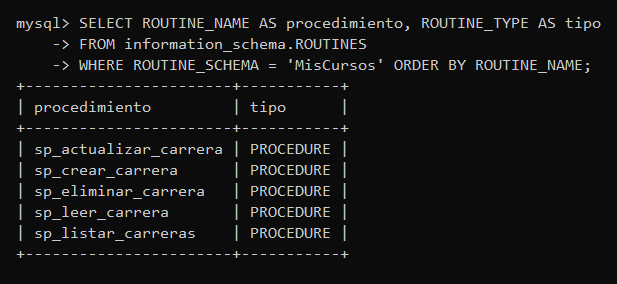
\includegraphics[width=0.65\linewidth]{10_procedimientos.png}
	\caption{Los cinco procedimientos almacenados creados en la base MisCursos}
	\label{img:procs}
\end{figure}

\begin{figure}[H]
	\centering
	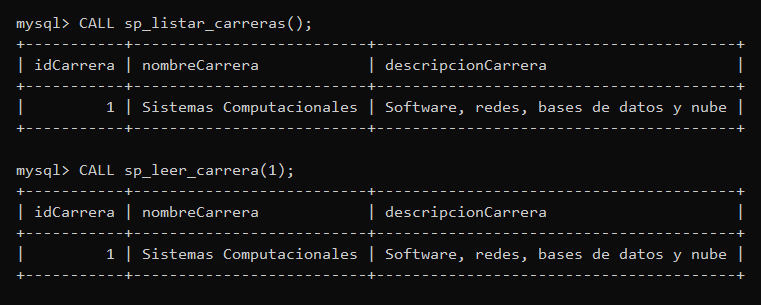
\includegraphics[width=0.85\linewidth]{11_llamadas_directas.png}
	\caption{Ejecución directa de dos procedimientos desde el cliente de MySQL}
	\label{img:calls}
\end{figure}

\subsection{Los métodos CRUD con CallableStatement}

Cada método del DAO abre una conexión, prepara la llamada con \texttt{prepareCall}, asigna los parámetros, ejecuta y cierra los recursos en un bloque \texttt{finally}. La sintaxis \texttt{\{call nombre(?, ?)\}} es la forma estándar de JDBC para invocar un procedimiento, independiente del manejador \cite{oracle_callablestatement}. Los signos de interrogación son los parámetros, que se asignan por posición empezando en 1 (\texttt{setString(1, ...)}, \texttt{setInt(1, ...)}).

\begin{lstlisting}[caption={Alta de una carrera: \texttt{create} llama a \texttt{sp\_crear\_carrera}}]
public void create(Carrera c) throws SQLException {
    obtenerConexion();
    CallableStatement cs = null;
    try {
        cs = conexion.prepareCall("{call sp_crear_carrera(?, ?)}");
        cs.setString(1, c.getNombreCarrera());
        cs.setString(2, c.getDescripcionCarrera());
        cs.execute();
    } finally {
        if (cs != null) cs.close();
        if (conexion != null) conexion.close();
    }
}
\end{lstlisting}

\texttt{update} y \texttt{delete} siguen el mismo esquema, con \texttt{sp\_actualizar\_carrera} (tres parámetros: id, nombre y descripción) y \texttt{sp\_eliminar\_carrera} (un parámetro: id). Los métodos de consulta cambian en un detalle: como sus procedimientos terminan en un \texttt{SELECT}, se ejecutan con \texttt{executeQuery()} y se recorre el \texttt{ResultSet}, en vez de \texttt{execute()}.

\begin{lstlisting}[caption={Consulta general: \texttt{readAll} llama a \texttt{sp\_listar\_carreras}}]
public List<Carrera> readAll() throws SQLException {
    obtenerConexion();
    CallableStatement cs = null;
    ResultSet rs = null;
    try {
        cs = conexion.prepareCall("{call sp_listar_carreras()}");
        rs = cs.executeQuery();
        return obtenerResultados(rs);
    } finally {
        if (rs != null) rs.close();
        if (cs != null) cs.close();
        if (conexion != null) conexion.close();
    }
}
\end{lstlisting}

El método privado \texttt{obtenerResultados} convierte cada fila del \texttt{ResultSet} en un objeto \texttt{Carrera}, y \texttt{read} reutiliza ese mismo método y devuelve el primer elemento, o \texttt{null} si no hubo filas.

\subsection{La interfaz gráfica y el CRUD completo}

La ventana arranca con solo \textbf{Nuevo} y \textbf{Listar} habilitados y la tabla vacía (figura \ref{img:inicial}). Con \textbf{Nuevo} se habilitan el formulario y \textbf{Guardar} (figura \ref{img:altaform}). Al guardar, \texttt{create()} inserta el registro y la tabla se refresca leyendo de nuevo con \texttt{readAll()} (figuras \ref{img:alta1} y \ref{img:alta2}).

\begin{figure}[H]
	\centering
	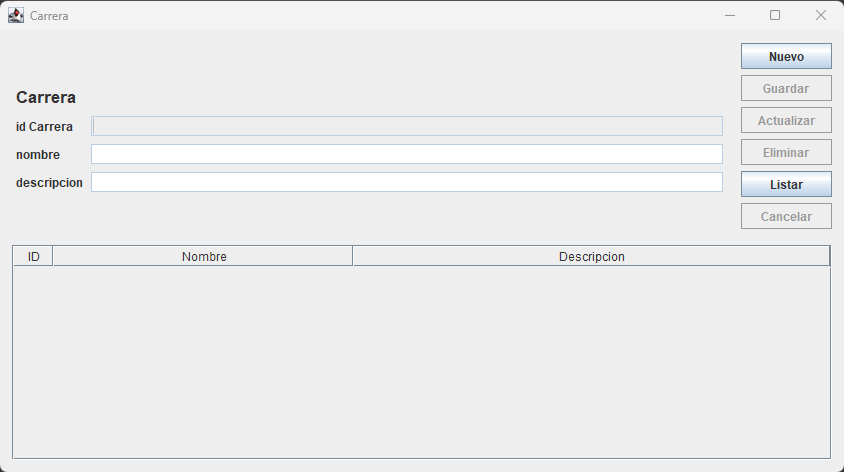
\includegraphics[width=0.95\linewidth]{01_estado_inicial.png}
	\caption{Estado inicial: solo Nuevo y Listar habilitados, tabla vacía}
	\label{img:inicial}
\end{figure}

\begin{figure}[H]
	\centering
	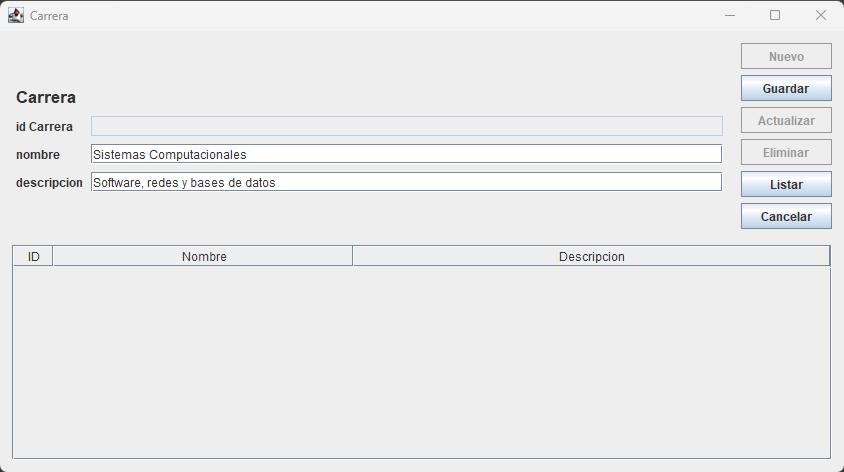
\includegraphics[width=0.95\linewidth]{02_alta_formulario.png}
	\caption{Alta: formulario lleno tras presionar Nuevo, con Guardar y Cancelar habilitados}
	\label{img:altaform}
\end{figure}

\begin{figure}[H]
	\centering
	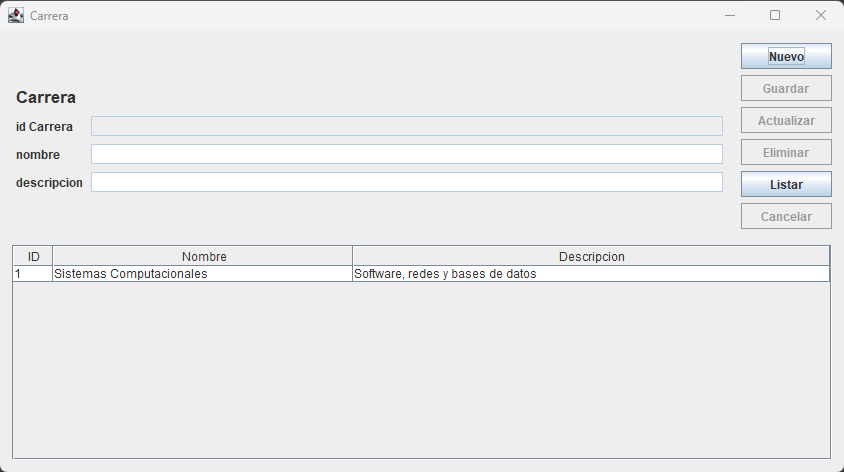
\includegraphics[width=0.95\linewidth]{03_alta_carrera1.png}
	\caption{Primera carrera guardada y leída de vuelta desde la base}
	\label{img:alta1}
\end{figure}

\begin{figure}[H]
	\centering
	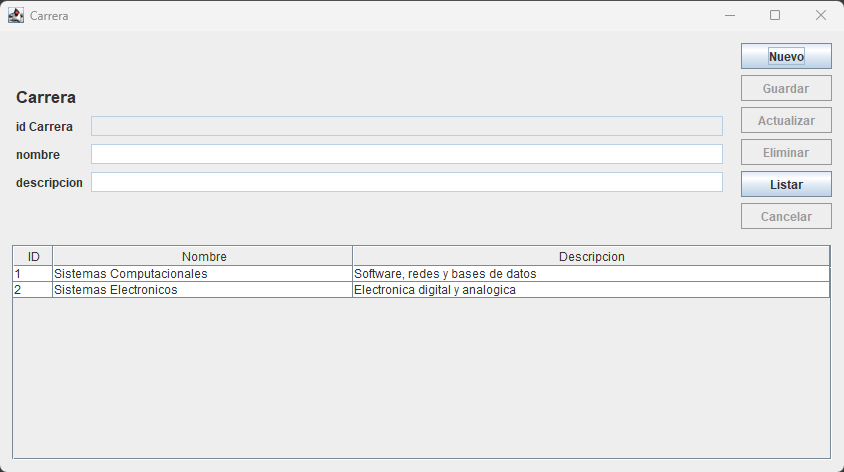
\includegraphics[width=0.95\linewidth]{04_alta_carrera2.png}
	\caption{Segunda alta: dos registros para probar cambio, baja y error}
	\label{img:alta2}
\end{figure}

Intentar dar de alta un nombre que ya existe hace que MySQL rechace el \texttt{INSERT} dentro del procedimiento. La excepción sube por el DAO hasta la ventana, que la muestra en un cuadro de error (figura \ref{img:duplicado}), y la tabla no cambia.

\begin{figure}[H]
	\centering
	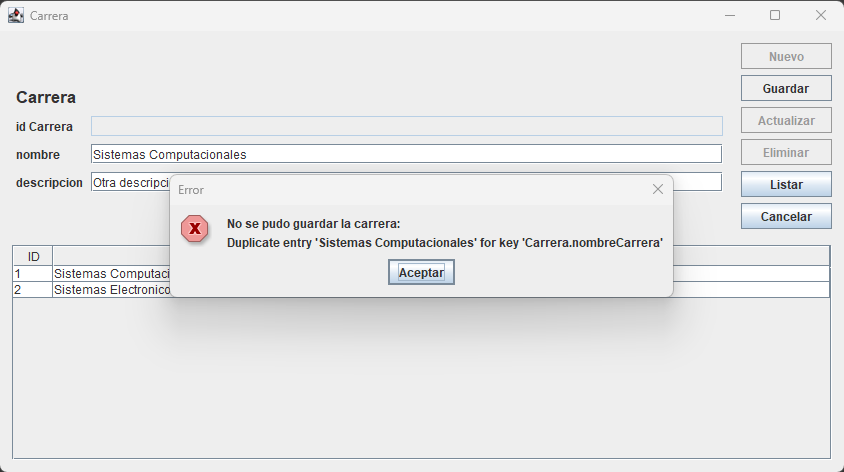
\includegraphics[width=0.95\linewidth]{05_error_duplicado.png}
	\caption{Error al repetir un nombre: restricción UNIQUE de nombreCarrera}
	\label{img:duplicado}
\end{figure}

Al seleccionar una fila se habilitan \textbf{Actualizar} y \textbf{Eliminar} y el formulario se llena con sus datos; el id queda de solo lectura (figura \ref{img:actform}). Tras editar la descripción y presionar \textbf{Actualizar}, \texttt{update()} llama a \texttt{sp\_actualizar\_carrera} y la tabla ya muestra el cambio (figura \ref{img:act}).

\begin{figure}[H]
	\centering
	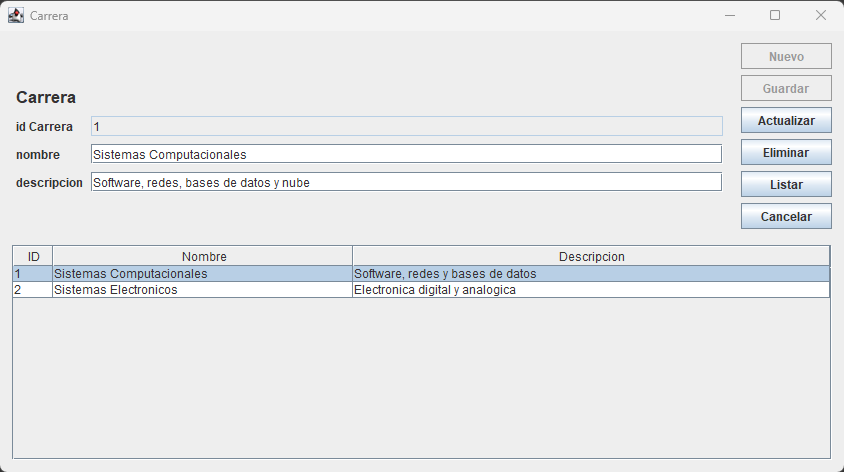
\includegraphics[width=0.95\linewidth]{06_actualizar_formulario.png}
	\caption{Carrera 1 seleccionada, con la descripción editada antes de Actualizar}
	\label{img:actform}
\end{figure}

\begin{figure}[H]
	\centering
	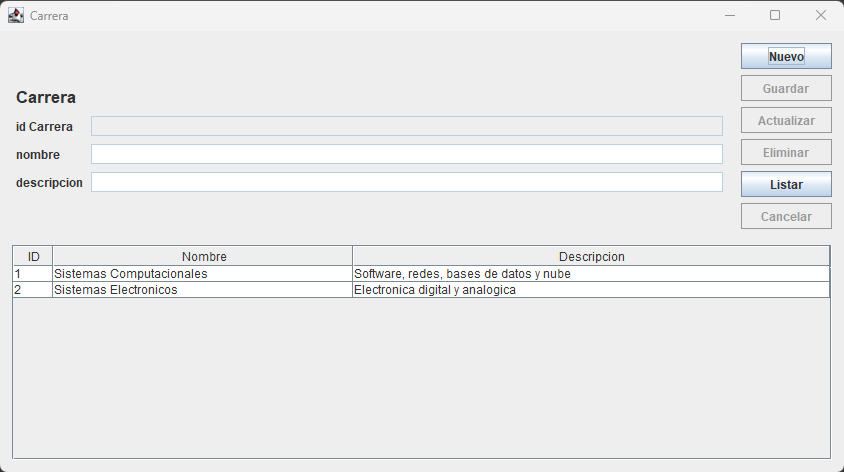
\includegraphics[width=0.95\linewidth]{07_actualizar_carrera1.png}
	\caption{Carrera 1 con la descripción actualizada}
	\label{img:act}
\end{figure}

Eliminar pide confirmación antes de llamar a \texttt{sp\_eliminar\_carrera} (figura \ref{img:confirmar}). Una vez confirmado, la fila desaparece porque la tabla se vuelve a leer de la base (figura \ref{img:final}).

\begin{figure}[H]
	\centering
	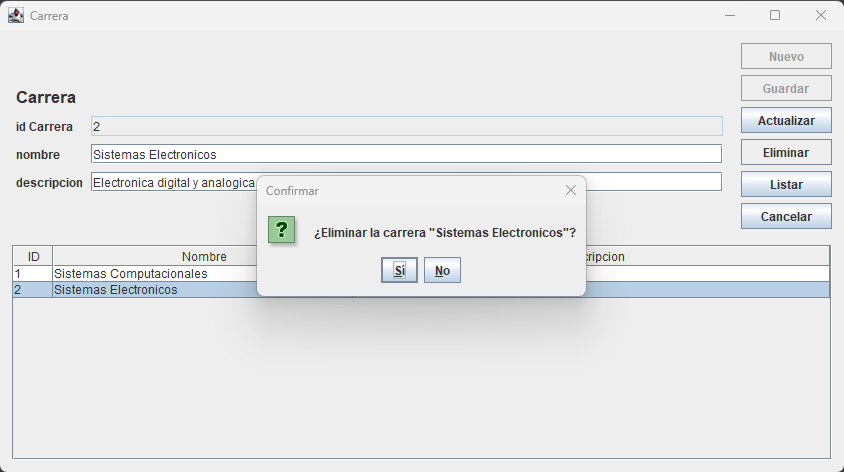
\includegraphics[width=0.95\linewidth]{08_confirmar_eliminar.png}
	\caption{Confirmación antes de eliminar la carrera 2}
	\label{img:confirmar}
\end{figure}

\begin{figure}[H]
	\centering
	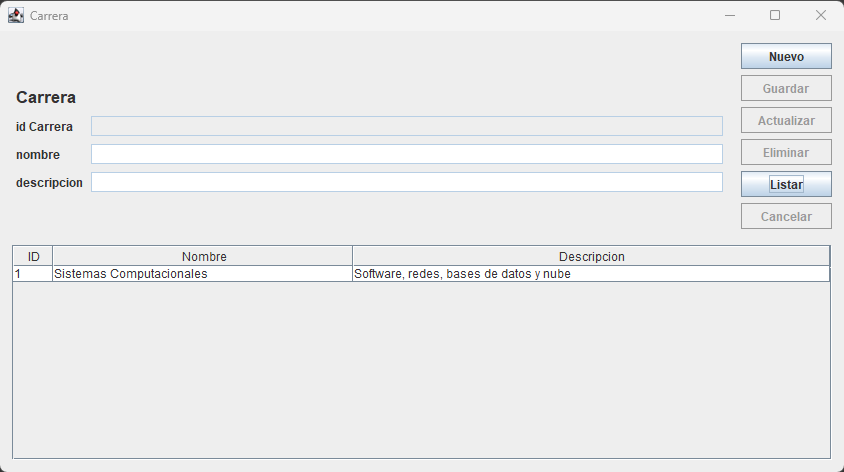
\includegraphics[width=0.95\linewidth]{09_estado_final.png}
	\caption{Estado final: solo queda la carrera 1, ya actualizada}
	\label{img:final}
\end{figure}

\subsection{Evidencia de la conexión JDBC y de las llamadas a los procedimientos}

Para comprobar que la interfaz llega hasta la base, y que lo hace a través de los procedimientos, se activó temporalmente el registro general de consultas de MySQL (\texttt{general\_log}) en el contenedor y se repitió toda la secuencia de las figuras anteriores. La figura \ref{img:jdbc} muestra el resultado. La primera consulta lista las conexiones que no vienen del propio contenedor: son las del DAO, que entran por TCP desde el equipo anfitrión (\texttt{172.19.0.1}) a la base \texttt{MisCursos}. Aparece más de una porque cada método del DAO abre y cierra su propia conexión en \texttt{obtenerConexion()}.

La segunda consulta lista lo que el servidor recibió con \texttt{CALL}. Cada acción de la ventana llegó como una llamada a un procedimiento: \texttt{sp\_crear\_carrera} en las altas, \texttt{sp\_actualizar\_carrera} en el cambio y \texttt{sp\_eliminar\_carrera} en la baja, cada una seguida de \texttt{sp\_listar\_carreras} para refrescar la tabla. La tercera llamada a \texttt{sp\_crear\_carrera}, con el nombre repetido, es el intento de la figura \ref{img:duplicado}: llegó al servidor pero no insertó nada. Las horas están en la zona horaria del contenedor (UTC). Al terminar se desactivó el registro y se vació.

\begin{figure}[H]
	\centering
	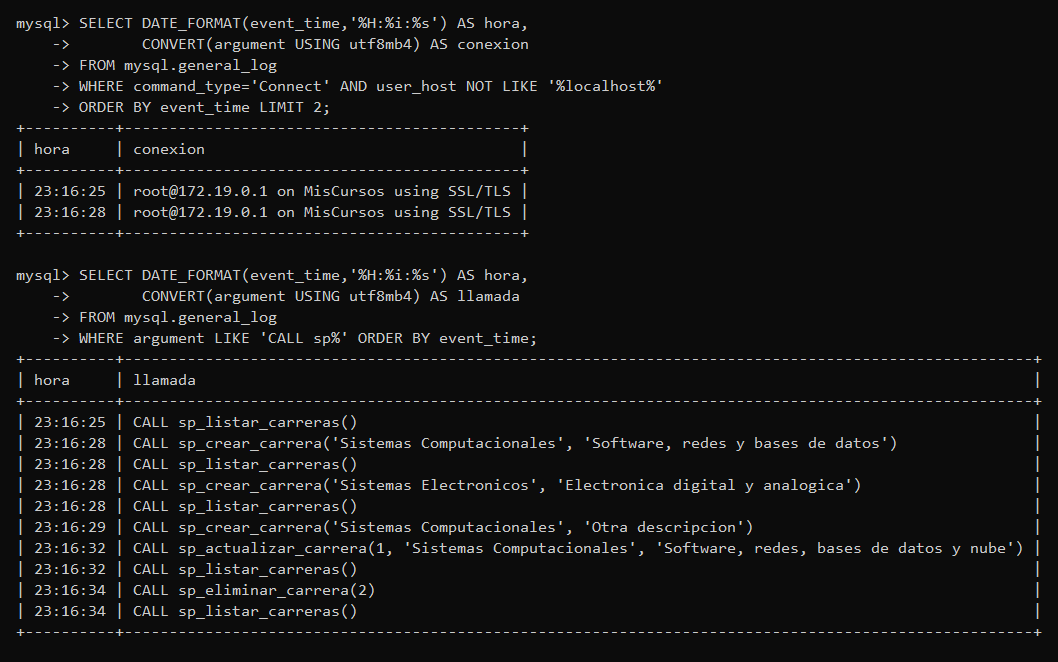
\includegraphics[width=\linewidth]{12_evidencia_jdbc.png}
	\caption{Registro del servidor: conexiones JDBC del DAO y llamadas a los procedimientos}
	\label{img:jdbc}
\end{figure}

Por último, la figura \ref{img:select} consulta la tabla directamente. El único registro y su descripción coinciden con el estado final de la ventana (figura \ref{img:final}).

\begin{figure}[H]
	\centering
	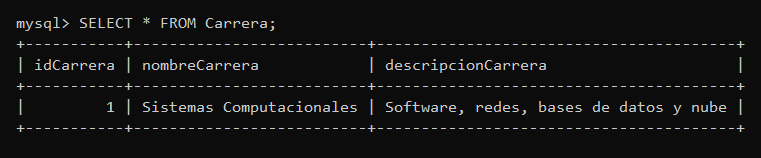
\includegraphics[width=0.85\linewidth]{13_select_final.png}
	\caption{Contenido real de la tabla tras las operaciones hechas desde la ventana}
	\label{img:select}
\end{figure}

%################################################
\section{\color{colorIPN}{Conclusiones}}

\textbf{Tipos de \textit{statement}.} JDBC ofrece tres: \texttt{Statement} (SQL como texto, sin parámetros), \texttt{PreparedStatement} (SQL con parámetros \texttt{?}, precompilado) y \texttt{CallableStatement}, que hereda del anterior y sirve para invocar procedimientos almacenados. Con \texttt{CallableStatement} el texto de la consulta en Java se reduce a \texttt{\{call sp\_x(?, ?)\}}: el SQL vive en el servidor y se puede cambiar sin recompilar la aplicación, aunque hay que instalar los procedimientos junto con la base. En esta práctica, la ventana y \texttt{Carrera} solo dependen de los cinco métodos del DAO, así que todo lo relacionado con los procedimientos queda contenido en \texttt{CarreraDAO}.

\textbf{Tipos de parámetros y de datos.} Un procedimiento puede declarar parámetros \texttt{IN}, \texttt{OUT} e \texttt{INOUT}. Los cinco de esta práctica son solo \texttt{IN}, así que basta con \texttt{setInt} y \texttt{setString}. Los parámetros \texttt{OUT} requieren registrarse antes de ejecutar con \texttt{registerOutParameter} \cite{mysql_connectorj_callable}. El tipo del \texttt{set} debe corresponder al de la columna (\texttt{INT} con \texttt{setInt}, \texttt{VARCHAR} con \texttt{setString}).

\textbf{Errores más típicos.} Casi todos llegan como \texttt{SQLException} o una de sus subclases. La tabla \ref{tab:errores} resume los que se pueden presentar con esta configuración. De ellos, solo el de nombre duplicado se reprodujo en la práctica (figura \ref{img:duplicado}); los demás se describen según la documentación y por cómo está armado el proyecto, sin haberse provocado.

\begin{table}[H]
	\centering
	\small
	\setlength{\tabcolsep}{4pt}
	\begin{tabular}{@{}>{\raggedright\arraybackslash}p{4.2cm}>{\raggedright\arraybackslash}p{6.0cm}>{\raggedright\arraybackslash}p{6.0cm}@{}}
		\toprule
		Error & Causa típica & Cómo se evita o se resuelve \\
		\midrule
		Nombre duplicado (\texttt{SQLIntegrity\allowbreak Constraint\allowbreak Violation\allowbreak Exception}) & Se repite \texttt{nombreCarrera}, que es \texttt{UNIQUE}. Es el que se vio en la figura \ref{img:duplicado}. & Capturar la excepción y avisar al usuario, como hace la ventana. \\
		Conexión rechazada o \textit{Access denied} & Contenedor apagado, puerto equivocado, o usuario o contraseña que no coinciden con los del contenedor. & Revisar que \texttt{docker ps} muestre el contenedor y que la URL, el usuario y la clave del DAO coincidan con el \texttt{docker-compose.yml}. \\
		Puerto equivocado & Este contenedor publica MySQL en el puerto 3307, no en el 3306 que es el habitual. Con la URL apuntando al 3306, la conexión se rechaza o llega a otro servidor MySQL del equipo. & Confirmar el puerto en la URL antes de ejecutar. \\
		El procedimiento no existe & Los scripts de \texttt{init/} solo corren cuando el contenedor se crea desde cero. Si la base ya existía, no se crean los procedimientos. & Ejecutar \texttt{02-procedimientos.sql} a mano, o recrear el contenedor. \\
		Número o tipo de parámetros incorrecto & Llamar \texttt{\{call sp\_crear\_carrera(?)\}} con dos valores, o usar \texttt{setInt} donde va \texttt{setString}. Los índices empiezan en 1, no en 0. & Que la firma de \texttt{prepareCall} coincida con la del procedimiento (tabla \ref{tab:correspondencia}). \\
		\texttt{execute} contra \texttt{executeQuery} & Usar \texttt{executeUpdate} con un procedimiento que devuelve filas, o \texttt{executeQuery} con uno que no devuelve nada. & \texttt{executeQuery} para \texttt{sp\_leer\_carrera} y \texttt{sp\_listar\_carreras}; \texttt{execute} para los otros tres. \\
		Falta \texttt{DELIMITER} al crear procedimientos & Sin cambiar el delimitador, el cliente corta el script en el primer \texttt{;} del cuerpo y el \texttt{CREATE PROCEDURE} queda incompleto. & Envolver el script con \texttt{DELIMITER \$\$} \dots{} \texttt{DELIMITER ;}. \\
		\texttt{ClassNotFoundException} & El conector de MySQL no está en el \textit{classpath}. & Incluir el \texttt{.jar} al compilar y al ejecutar; el DAO lo convierte en \texttt{SQLException}. \\
		Recursos sin cerrar & Conexiones y \texttt{CallableStatement} abiertos si ocurre una excepción antes del \texttt{close()}. & Cerrarlos en \texttt{finally}, como hacen los cinco métodos. \\
		\bottomrule
	\end{tabular}
	\caption{Errores típicos al trabajar con JDBC, DAO y procedimientos almacenados}
	\label{tab:errores}
\end{table}

El DAO conserva su estructura; lo que envía ahora es una llamada en lugar de una consulta. El costo es que el nombre y los parámetros del procedimiento en la base deben coincidir con la cadena \texttt{\{call ...\}} en Java.

%################################################
\section{\color{colorIPN}{Referencias Bibliográficas}}
\nocite{*}
\color{colorESCOM}{
	\printbibliography[heading=none]
}

\end{document}
